\chapter{Tranzystor fet z kanałem grafenowym}
	Idea tranzystora polowego zrodziła się już pierwszej połowie zeszłego stulecia. 
Natomiast dzisiejsze znaczenie tranzystory polowe uzyskały dzięki tranzystorowi
typu MOSFET wynalezionemu w 1960 roku przez  Dawon Kahng i Martin Atalla. 
Dzięki ich wynalazkowi elektronika rozpoczęła swoją ekspansję w każdą dziedzinę
naszego życia.
	
\section{Zasada działania}

	\begin{wrapfigure}{r}{0.5\textwidth}
	\begin{center}
	    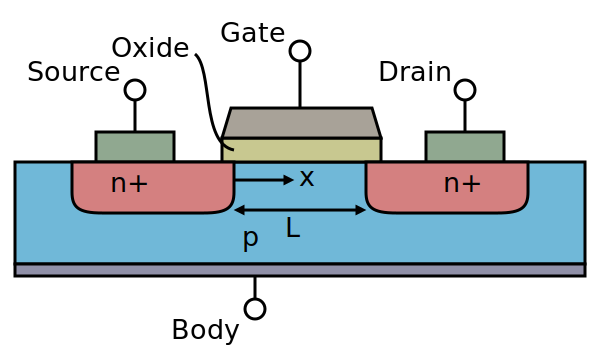
\includegraphics[width=0.48\textwidth]{./Rozdzial_2/obrazki/Lateral_mosfet}
	  \end{center}
 	 \caption{Schemat budowy tranzystora typu MOS}
	\label{fig:budowa_tranzystora_MOS}
	\end{wrapfigure}


	Typowa budowa tranzystora typu MOSFET została przedstawiona na rysunku \ref{fig:budowa_tranzystora_MOS}.
Taki tranzystor składa

Tutaj opis dla typowego mosa, wraz z opisami stanów w jakich może się znajdować
półprzewodnik kanału.	
	
	
\section{Grafen i jego właściwości}
	wiązania->struktura sieci->pasma->ruchliwość->koncentracja->wpływ oddziaływania
z podłożem na powyższe właściwości->wpływ domieszkowania na strukturę pasmową->
wpływ środowiska

	\section{Tranzystor polowy z kanałem grafenowym}
	
	charakterystyki elektryczne dla różnych konfiguracji i ich omówienie.
	Brak podziału na 3 obszary pracy kanału. Tylko jeden zawsze.
